% =============================================================================
% KAPITEL 5: MODELLIERUNG UND IMPLEMENTIERUNG
% =============================================================================

\chapter{Modellierung und Implementierung}\label{chap:modellierung}

Dieses Kapitel beschreibt die konkrete Umsetzung der in Kapitel~\ref{chap:methodik}
entworfenen Pipeline. Die gesamte Implementierung ist in zwei Python-Dateien
organisiert: \texttt{utils.py} enthält die wiederverwendbare Datenpipeline und
das Feature Engineering, \texttt{notebook.ipynb} die explorative Datenanalyse,
die Konstruktion der Datensatzvarianten sowie das Training und die Evaluation
aller Modelle. Abschnitt~\ref{sec:datengrundlage} beschreibt die Rohdaten
und deren Aufbereitung. Abschnitt~\ref{sec:feature-engineering-impl} erläutert
das Feature Engineering vom Laden der Daten bis zur finalen Feature-Liste.
Abschnitt~\ref{sec:umsetzung} dokumentiert die vollständige
Modellierungspipeline von der Variantendefinition über das Hyperparameter-Tuning
bis zur Modellspeicherung.

% =============================================================================
\section{Datengrundlage}
\label{sec:datengrundlage}
% =============================================================================

\subsection{Übersicht der Datenquellen}

Die Implementierung stützt sich auf zwei unabhängige Datenquellen, die jeweils
zehn Bundesliga-Saisons von 2016/17 bis 2025/26 abdecken. Die
\textbf{Bundesliga-Spieldaten} stammen aus dem Verzeichnis
\texttt{Bundesliga\_Quellen/} und enthalten Match-Level-Informationen zu
jedem Spiel. Die \textbf{xG-Saisondaten} aus \texttt{xG\_Quellen/} liefern
teamspezifische Expected-Goals-Statistiken je Saison, bereitgestellt von
Understat \cite{Understat2024}. Beide Quellen liegen im CSV-Format vor
und werden über die Bibliothek \texttt{pandas} \cite{McKinney2010} eingelesen.

\subsection{Laden der Bundesliga-Spieldaten}

Das Laden aller Bundesliga-Daten übernimmt die Funktion
\texttt{load\_bundesliga\_data()} in \texttt{utils.py}. Sie iteriert über
alle CSV-Dateien im Bundesliga-Verzeichnis und wendet dabei zwei bewusste
Designentscheidungen um:

\begin{lstlisting}[language=Python, caption={Kernauszug aus \texttt{load\_bundesliga\_data()}},
                   label={lst:load-bundesliga}]
files = sorted(glob.glob(os.path.join(BUNDESLIGA_DIR, "*.csv")))
for f in files:
    try:
        df = pd.read_csv(f, encoding="utf-8", on_bad_lines="skip")
    except Exception:
        df = pd.read_csv(f, encoding="latin-1", on_bad_lines="skip")

    df["Season"] = _parse_season_label(f)
    df = df.dropna(subset=["HomeTeam", "AwayTeam", "FTR"])
    df["HomeTeam"] = df["HomeTeam"].apply(normalize_team)
    df["AwayTeam"] = df["AwayTeam"].apply(normalize_team)
    df["Date"] = pd.to_datetime(df["Date"], dayfirst=True, errors="coerce")
\end{lstlisting}

Erstens wird zunächst UTF-8-Kodierung versucht; schlägt dies fehl, wird
automatisch auf Latin-1 zurückgefallen, da ältere Datensätze teilweise
in Latin-1 kodiert sind. Zweitens extrahiert \texttt{\_parse\_season\_label()}
die Saisonbezeichnung direkt aus dem Dateinamen -- \texttt{Bundesliga 2016-2017.csv}
ergibt \texttt{2016/17}. Nach dem Zusammenführen werden Zeilen mit
unzulässigen FTR-Werten verworfen und numerische Spalten explizit in
\texttt{float} konvertiert. Der vollständige Bereinigungscode findet sich
in Anhang~\ref{app:code} (Listing~\ref{lst:load-clean}).

\subsection{Teamnamen-Normalisierung}

Ein zentrales Problem bei der Zusammenführung beider Datenquellen ist die
inkonsistente Schreibweise von Teamnamen: Borussia Dortmund erscheint in
den Bundesliga-CSVs als \texttt{"Dortmund"}, in den xG-Dateien hingegen
als \texttt{"Borussia Dortmund"}. Die Lösung ist das Dictionary
\texttt{TEAM\_NAME\_MAP} in \texttt{utils.py}, das alle bekannten
Schreibvarianten aller 36 vorkommenden Vereine auf eine einheitliche
Zielform abbildet (Anhang~\ref{app:code}, Listing~\ref{lst:normalize}).
Trifft \texttt{normalize\_team()} auf einen unbekannten Namen, gibt es
diesen unverändert zurück -- ein bewusst defensives Vorgehen, das sicherstellt,
dass neue Aufsteiger nicht stillschweigend verworfen werden.

\subsection{Laden der xG-Saisondaten}

Die xG-Daten werden über \texttt{load\_xg\_data()} geladen. Die wichtigste
Transformation ist die Normierung der Summenwerte auf einen
Per-Spiel-Durchschnitt durch Division durch \texttt{matches}
(Listing~\ref{lst:load-xg} im Anhang). Dies ist notwendig, da
Saisonsummen bei unterschiedlich vielen Spielen je Team nicht direkt
vergleichbar sind -- etwa bei Auf- und Absteigern \cite{AnzerBauer2021}.

\subsection{Explorative Datenanalyse}

Nach dem Laden der Daten werden im Notebook mehrere explorative Analysen
durchgeführt, die Modellierungsentscheidungen motivieren.

\subsubsection{Verteilung der Zielvariable}

\begin{figure}[h]
    \centering
    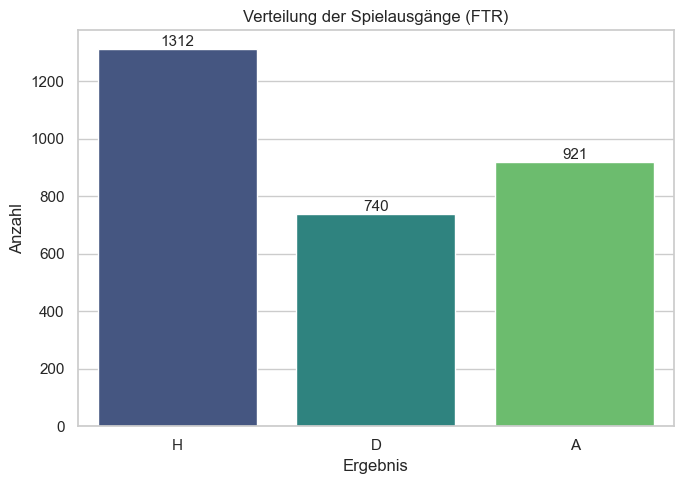
\includegraphics[width=0.6\textwidth]{plots/plot_ftr_verteilung.png}
    \caption{Verteilung der Spielausgänge (FTR) im bereinigten Datensatz.
             Heimsiege (H) dominieren mit rund 45\,\%, gefolgt von
             Auswärtssiegen (A) mit ca.\ 30\,\% und Unentschieden (D)
             mit rund 25\,\%.}
    \label{fig:ftr-verteilung}
\end{figure}

Abbildung~\ref{fig:ftr-verteilung} zeigt die Ungleichverteilung der
drei Klassen. Der Heimvorteil führt dazu, dass Heimsiege die häufigste
Klasse sind, während Unentschieden die seltenste darstellen. Diese
Klassen-Imbalance ist der Hauptgrund, warum Macro-F1 statt Accuracy als
primäre Evaluationsmetrik verwendet wird \cite{HeGarcia2009}.

\subsubsection{Korrelationsanalyse}

Für die Korrelationsanalyse wird \texttt{FTR} numerisch kodiert
(\texttt{H}~=~+1, \texttt{D}~=~0, \texttt{A}~=~-1), um den
Pearson-Korrelationskoeffizienten zwischen jedem Feature und der
Zielvariable zu berechnen \cite{JamesEtAl2021}. Der zugehörige Code
findet sich in Anhang~\ref{app:code} (Listing~\ref{lst:korr}).

\begin{figure}[h]
    \centering
    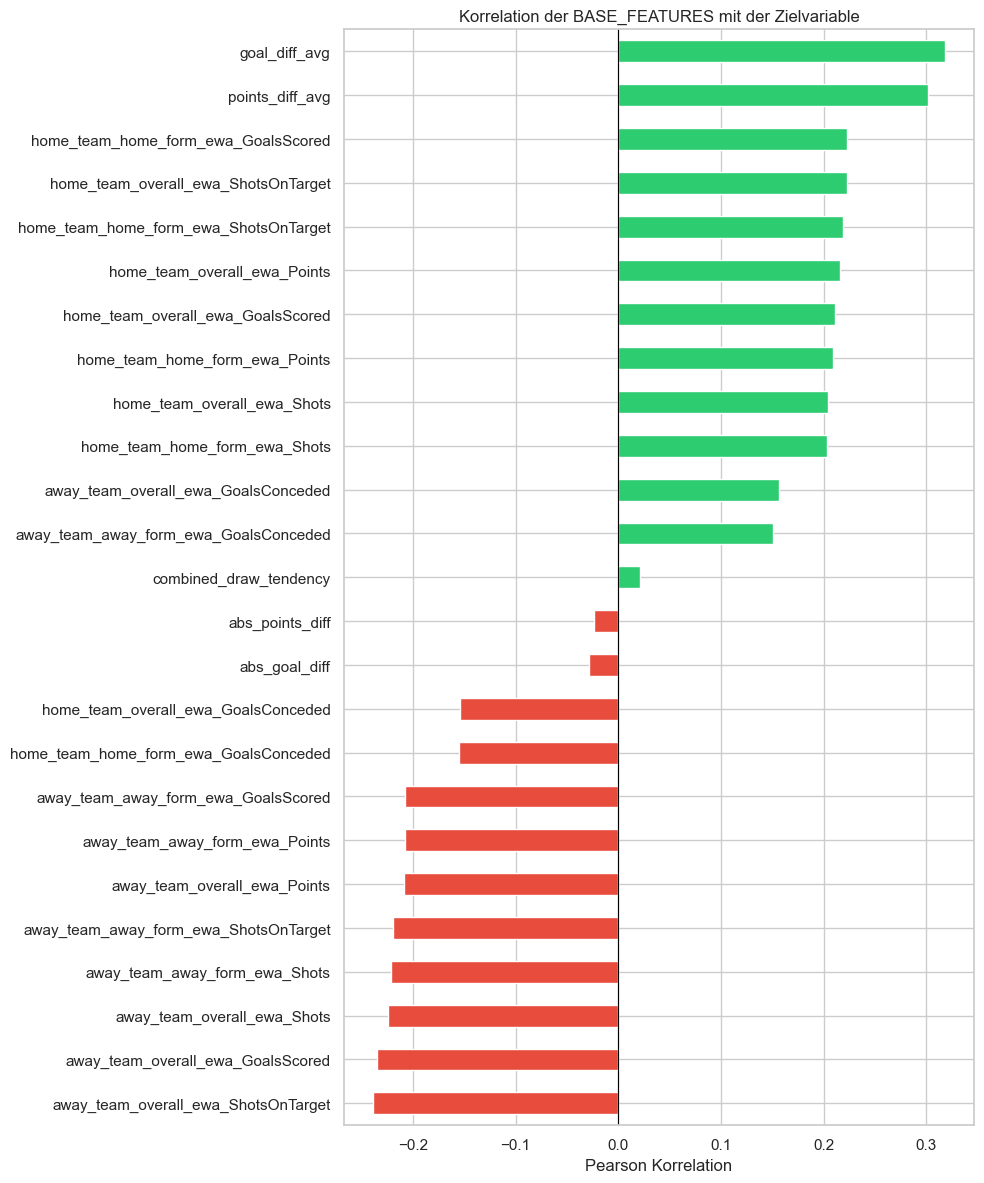
\includegraphics[width=\textwidth]{plots/plot_korrelation_target.png}
    \caption{Pearson-Korrelation aller BASE\_FEATURES mit der Zielvariable
             \texttt{Target\_Heimerfolg}. Positive Korrelation (grün)
             indiziert eine Begünstigung des Heimsiegs, negative Korrelation
             (rot) eine Begünstigung des Auswärtssiegs.}
    \label{fig:korrelation-target}
\end{figure}

Abbildung~\ref{fig:korrelation-target} zeigt, dass punktebezogene
EWA-Features die stärksten Korrelationen mit dem Heimerfolg aufweisen --
insbesondere \texttt{points\_diff\_avg} und
\texttt{home\_team\_overall\_ewa\_Points}.
Dieses Ergebnis motiviert die spätere Feature-Selektion mit einem
Schwellenwert von $|\,r\,| > 0{,}1$.

% =============================================================================
\section{Feature Engineering}
\label{sec:feature-engineering-impl}
% =============================================================================

\subsection{Konzept und Überblick}

Das Feature Engineering ist das methodische Herzstück der Implementierung.
Rohe Spielstatistiken -- Tore, Schüsse, Ergebnis -- sind für ein
Machine-Learning-Modell ohne Kontextualisierung wenig aussagekräftig:
Das Ergebnis eines einzelnen Spiels ist stark zufallsbehaftet, während
die Teamform über mehrere Spiele hinweg ein stabileres Signal liefert
\cite{Wheatcroft2022}. Die zentrale Funktion \texttt{compute\_rolling\_features()}
in \texttt{utils.py} ergänzt den DataFrame um 20 EWA-basierte Form-Features.

\subsection{Transformation ins Team-Spiel-Format}

Als erstes wird jedes Spiel in zwei Beobachtungen aufgeteilt: eine
aus Perspektive des Heimteams, eine aus Perspektive des Auswärtsteams
(Listing~\ref{lst:longformat} im Anhang). Dabei werden die Spalten für
das Auswärtsteam konsequent umgepolt: \texttt{FTAG} wird zu
\texttt{GoalsScored}, \texttt{FTHG} zu \texttt{GoalsConceded} -- da aus
Sicht des Gastes die gegnerischen Tore die eigenen Gegentore sind. Dies
stellt sicher, dass \texttt{GoalsScored} und \texttt{GoalsConceded} über
alle Teams hinweg eine einheitliche semantische Bedeutung haben.

\subsection{Punkteberechnung}

Aus dem langen Format werden teamspezifische Punktwerte berechnet: drei
Punkte für einen Sieg, einer für ein Unentschieden, null für eine Niederlage
-- jeweils aus Teamperspektive (Anhang~\ref{app:code},
Listing~\ref{lst:punkte}).

\subsection{EWA-Berechnung mit Shift-Operation}

Die eigentliche EWA-Berechnung erfolgt in der inneren Funktion
\texttt{compute\_ewa()}. Die kritischste Zeile ist dabei die
\texttt{.shift(1)}-Operation:

\begin{lstlisting}[language=Python, caption={Kern der EWA-Berechnung mit Anti-Leakage-Shift},
                   label={lst:ewa-kern}]
def compute_ewa(data, span):
    grouped = data.groupby("Team")
    # shift(1): nur VERGANGENE Spiele einfliessen lassen
    shifted = grouped.shift(1)
    ewa = (shifted[["GoalsScored","GoalsConceded",
                     "Points","Shots","ShotsOnTarget"]]
           .groupby(data["Team"])
           .ewm(span=span, min_periods=1)
           .mean())
    ewa = ewa.reset_index(level=0, drop=True)
    return ewa
\end{lstlisting}

\textbf{Warum \texttt{.shift(1)}?} Ohne diese Verschiebung würde der
EWA-Wert für Spiel $t$ das Ergebnis von Spiel $t$ selbst beinhalten.
Das Modell hätte damit implizit Zugang zum Ergebnis des Spiels, das es
vorhersagen soll -- ein klassisches Data-Leakage-Problem
\cite{KaufmanRossetPerlich2012}. Durch \texttt{.shift(1)} wird
sichergestellt, dass ausschließlich die Statistiken
\emph{vorangegangener} Spiele einfließen. Die EWA selbst wird mit
\texttt{.ewm(span=10, min\_periods=1).mean()} berechnet; der
Glättungsfaktor beträgt $\alpha = \frac{2}{11} \approx 0{,}182$.

\subsection{Drei EWA-Kontexte}

Die EWA-Berechnung wird in drei separaten Kontexten durchgeführt
(Listing~\ref{lst:drei-kontexte} im Anhang):
\texttt{overall\_ewa} über alle Spiele, \texttt{home\_form\_ewa}
ausschließlich über Heimspiele des Heimteams, und \texttt{away\_form\_ewa}
ausschließlich über Auswärtsspiele des Auswärtsteams. Diese Trennung
ist durch Befunde motiviert, die zeigen, dass Heim- und Auswärtsform
unterschiedliche Stabilitätseigenschaften aufweisen \cite{DobsonGoddard2011}.
Pro Kontext werden fünf Metriken berechnet, was in $3 \times 5 \times 2 = 30$
Feature-Spalten resultiert, die auf 20 reduziert werden, da
\texttt{home\_form\_ewa} nur für das Heimteam und
\texttt{away\_form\_ewa} nur für das Auswärtsteam genutzt wird. Die
anschließende Rückführung in den Match-Level-DataFrame erfolgt über
einen Daten-Join auf \texttt{Date} und \texttt{Team} mit dem
Präfix-Schema \texttt{home\_team\_*} / \texttt{away\_team\_*}
(Listing~\ref{lst:merge-ewa} im Anhang).

\subsection{Abgeleitete Differenz-Features}

Nach der EWA-Berechnung werden fünf weitere Features als Differenzen
konstruiert (Anhang~\ref{app:code}, Listing~\ref{lst:diff-features}).
\texttt{goal\_diff\_avg} und \texttt{points\_diff\_avg} quantifizieren
den relativen Stärkevorteil des Heimteams; ihre Absolutwerte
\texttt{abs\_goal\_diff} und \texttt{abs\_points\_diff} messen die
Ausgeglichenheit beider Teams. Der \texttt{combined\_draw\_tendency}-Index
kombiniert beide Absolutwerte multiplikativ: Je kleiner die Differenzen,
desto höher der Index und desto wahrscheinlicher ein Unentschieden --
eine gezielte Reaktion auf die bekannte Schwäche von ML-Modellen bei
dieser Klasse \cite{HeGarcia2009,ChawlaEtAl2002}.

\subsection{xG-Integration mit Lag-1-Strategie}

Die xG-Daten werden in \texttt{merge\_xg\_features()} über eine
Lag-1-Strategie integriert, um Data Leakage zu verhindern:

\begin{lstlisting}[language=Python, caption={Lag-1-Strategie in \texttt{merge\_xg\_features()}},
                   label={lst:lag1}]
all_seasons = sorted(xg_slim["Season"].unique())
max_season  = all_seasons[-1]  # aktuelle/letzte Saison

rows = []
for i, s in enumerate(all_seasons):
    prior = all_seasons[i - 1] if i > 0 else s
    # Aktuelle Saison: direkte Nutzung. Historisch: Vorjahr.
    join_season = s if s == max_season else prior

    s_data = xg_slim[xg_slim["Season"] == join_season].copy()
    s_data["MatchSeason"] = s
    rows.append(s_data)

xg_mapped = pd.concat(rows, ignore_index=True)
\end{lstlisting}

Für jede historisch abgeschlossene Saison $s$ werden die xG-Werte der
Vorsaison $s-1$ als Prior verwendet, da Saisonendstatistiken erst nach
dem letzten Spieltag feststehen. Nur für die aktuelle Saison werden
die laufenden Werte direkt genutzt. Der anschließende Join auf
\texttt{HomeTeam}/\texttt{AwayTeam} und \texttt{Season} erfolgt separat
für Heim- und Auswärtsteam (Anhang~\ref{app:code}, Listing~\ref{lst:xg-join}).
Da für die erste Saison (2016/17) keine Vorsaison-xG vorliegen, enthält
der xG-Datensatz mit $\sim$2.280 Spielen weniger Beobachtungen als der
Basisdatensatz ($\sim$2.955 Spiele).

\subsection{Finale Feature-Sets}

Die beiden Feature-Listen sind als Konstanten in \texttt{utils.py}
definiert (vollständige Definition: Anhang~\ref{app:code},
Listing~\ref{lst:feature-sets}).
Tabelle~\ref{tab:feature-sets-impl} fasst die Zusammensetzung zusammen.

\begin{table}[h]
    \centering
    \caption{Zusammensetzung der Feature-Sets}
    \label{tab:feature-sets-impl}
    \begin{tabular}{l r r}
        \toprule
        \textbf{Feature-Gruppe} & \textbf{BASE} & \textbf{XG} \\
        \midrule
        Overall EWA Heimteam (5 Metriken)          & 5  & 5  \\
        Heimform EWA Heimteam (5 Metriken)         & 5  & 5  \\
        Overall EWA Auswärtsteam (5 Metriken)      & 5  & 5  \\
        Auswärtsform EWA Auswärtsteam (5 Metriken) & 5  & 5  \\
        Differenz-Features                         & 5  & 5  \\
        xG-basierte Features (6 + 3 Diff.)         & 0  & 9  \\
        \midrule
        \textbf{Gesamt}                            & \textbf{25} & \textbf{34} \\
        \bottomrule
    \end{tabular}
\end{table}

% =============================================================================
\section{Umsetzung}
\label{sec:umsetzung}
% =============================================================================

\subsection{Kodierung der Zielvariable}

Die kategorische Zielvariable \texttt{FTR} wird über
\texttt{sklearn}'s \texttt{LabelEncoder} in ganzzahlige Klassenindizes
überführt: \texttt{A}~→~0, \texttt{D}~→~1, \texttt{H}~→~2
(Listing~\ref{lst:labelencoder} im Anhang). Entscheidend ist, dass
\texttt{fit\_transform} ausschließlich auf \texttt{df\_base} angewendet
wird; \texttt{df\_with\_xg} wird nur mit \texttt{transform} ohne erneutes
Fitting transformiert, um dasselbe Klassenindex-Mapping zu gewährleisten.

\subsection{Konstruktion der Datensatzvarianten}

\subsubsection{Ausreißerbereinigung (IQR)}

Die Funktion \texttt{remove\_outliers\_iqr()} entfernt Beobachtungen
außerhalb von $[Q_1 - c \cdot \text{IQR},\; Q_3 + c \cdot \text{IQR}]$
(Anhang~\ref{app:code}, Listing~\ref{lst:iqr}). Der Multiplikator
$c = 3{,}0$ -- statt des üblicheren $c = 1{,}5$ -- wurde bewusst
konservativ gewählt: Bei EWA-geglätteten Features sind extreme Ausreißer
selten; ein strengerer Wert würde zu viele informationsreiche
Randbeobachtungen entfernen \cite{JamesEtAl2021}.

\subsubsection{Feature-Selektion via Korrelation}

\texttt{get\_strong\_features()} behält nur Features mit einem absoluten
Pearson-Korrelationskoeffizienten $|\,r\,| > 0{,}1$ zur numerisch
kodierten Zielvariable (Listing~\ref{lst:feature-sel} im Anhang). Dieser
Schwellenwert ist als konservative untere Schranke gewählt: Features
unterhalb davon tragen kaum zur Trennbarkeit der Klassen bei
\cite{JamesEtAl2021}.

\subsubsection{PCA-Varianten}

\texttt{apply\_pca()} führt eine PCA durch, die auf 95\,\% erklärter
Varianz beschränkt wird (Listing~\ref{lst:pca-impl} im Anhang). Der
\texttt{StandardScaler} wird dabei ausschließlich auf den aktuellen
Daten gefittet; \texttt{sklearn}'s PCA interpretiert
\texttt{n\_components=0.95} automatisch als Varianzanteil
\cite{ScikitLearn2024}.

\begin{figure}[h]
    \centering
    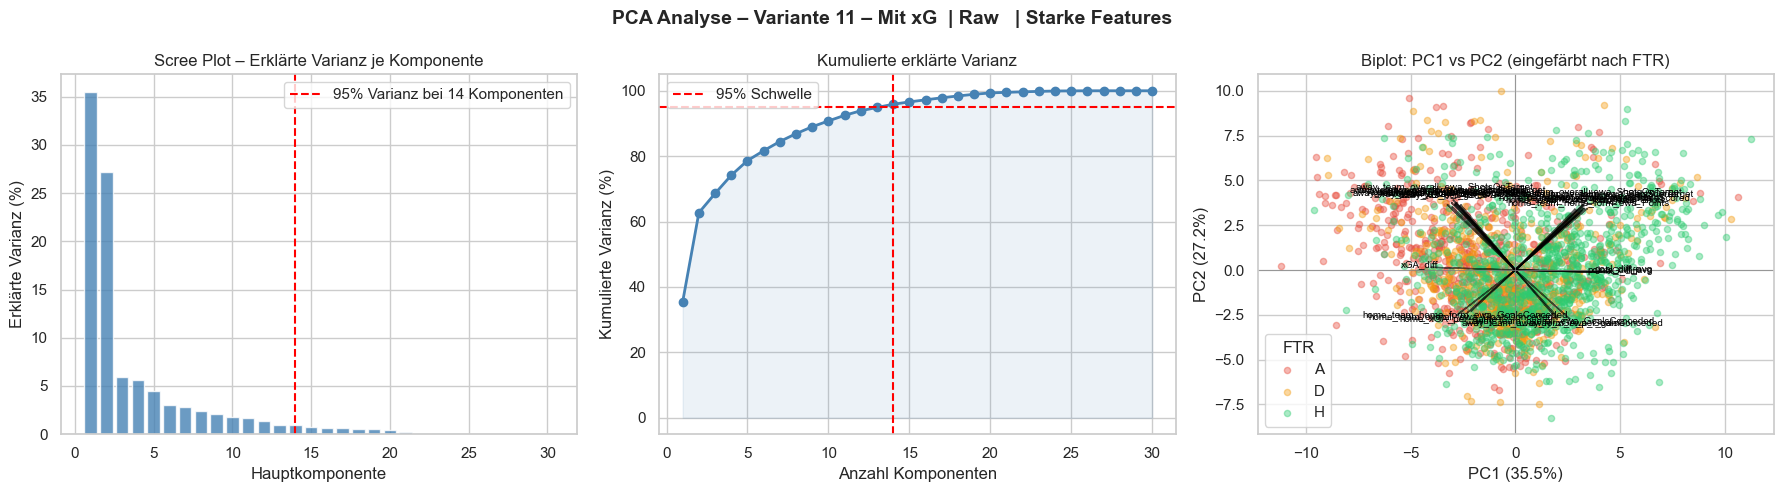
\includegraphics[width=\textwidth]{plots/plot_pca_analyse.png}
    \caption{PCA-Analyse für Variante~11 (Mit xG, Raw, Starke Features):
             Scree Plot (links), kumulierte erklärte Varianz mit
             95\,\%-Schwelle (Mitte) und Biplot der ersten zwei
             Hauptkomponenten eingefärbt nach Spielausgang (rechts).}
    \label{fig:pca-analyse}
\end{figure}

Im Biplot (Abbildung~\ref{fig:pca-analyse}, rechts) ist erkennbar, dass
die drei Klassen auch in der zweidimensionalen PCA-Projektion keine
klare lineare Trennbarkeit aufweisen -- ein Beleg für die inhärente
Schwierigkeit des Vorhersageproblems \cite{Sumpter2016}.

\subsubsection{Übersicht der zwölf Varianten}

Aus der kombinatorischen Verknüpfung der drei Achsen entstehen zwölf
Datensatzvarianten, die im Dictionary \texttt{variants} gespeichert werden
(vollständige Definition: Anhang~\ref{app:code}, Listing~\ref{lst:varianten}).
Die PCA-Varianten (9--12) sind strukturell konsistente Entsprechungen
der Starke-Feature-Varianten 2, 4, 6 und 8.

\subsection{Die Training-Pipeline: \texttt{run\_variant()}}

Alle 60 Trainingsläufe (12 Varianten $\times$ 5 Modelle) werden über
die gemeinsame Wrapper-Funktion \texttt{run\_variant()} durchgeführt:

\begin{lstlisting}[language=Python, caption={\texttt{run\_variant()}: gemeinsamer Trainings-Wrapper},
                   label={lst:run-variant}]
def run_variant(df_var, features):
    X = df_var[features].values
    y = df_var['Target'].values

    X_train, X_test, y_train, y_test = train_test_split(
        X, y, test_size=0.2, random_state=42, stratify=y)

    scaler  = StandardScaler()
    X_train = scaler.fit_transform(X_train)
    X_test  = scaler.transform(X_test)

    logreg_res = tune_logreg(X_train, X_test, y_train, y_test)
    rf_res     = tune_randomforest(X_train, X_test, y_train, y_test)
    lgbm_res   = tune_lightgbm(X_train, X_test, y_train, y_test)
    xgb_res    = tune_xgboost(X_train, X_test, y_train, y_test)
    mlp_res    = tune_mlp(X_train, X_test, y_train, y_test)

    return (logreg_res, rf_res, lgbm_res, xgb_res, mlp_res,
            scaler, X_test, y_test)
\end{lstlisting}

Zwei Design-Entscheidungen sind hier zentral. Der \texttt{StandardScaler}
wird mit \texttt{fit\_transform} ausschließlich auf dem Trainingsdatensatz
angepasst -- ein globales Fitten würde Testset-Statistiken einbeziehen
und stellt damit Data Leakage dar \cite{HastieEtAl2009}. Das
\texttt{stratify=y} im Train-Test-Split stellt sicher, dass die
Klassenverteilung im Testset proportional zur des Gesamtdatensatzes ist
\cite{JamesEtAl2021}.

\subsection{Hyperparameter-Tuning je Algorithmus}

Alle fünf Algorithmen werden über \texttt{RandomizedSearchCV} mit
\texttt{StratifiedKFold} (5 Folds) und F1-macro als Optimierungsmetrik
abgestimmt. Die vollständigen Suchräume aller Modelle sind in
Anhang~\ref{app:code} (Listings~\ref{lst:logreg-tuning}--\ref{lst:xgb-tuning})
dokumentiert.

\textbf{Klassen-Imbalance:} Logistische Regression und Random Forest
nutzen \texttt{class\_weight=`balanced'}. LightGBM und XGBoost erhalten
per \texttt{compute\_sample\_weight()} berechnete Sample-Weights beim
Fit-Aufruf, da sie kein direktes \texttt{class\_weight}-Argument
unterstützen.

\textbf{MLP -- manuelles Oversampling:} Da \texttt{MLPClassifier}
weder \texttt{class\_weight} noch \texttt{sample\_weight} unterstützt,
wird die Klassen-Imbalance durch manuelles Oversampling behoben:

\begin{lstlisting}[language=Python, caption={Manuelles Oversampling für das MLP},
                   label={lst:mlp-oversampling}]
class_counts = Counter(y_train)
max_count    = max(class_counts.values())

X_resampled, y_resampled = [X_train_df], [y_train_s]
for cls, count in class_counts.items():
    if count < max_count:
        deficit   = max_count - count
        idx       = y_train_s[y_train_s == cls].index
        extra_idx = np.random.choice(idx, size=deficit, replace=True)
        X_resampled.append(X_train_df.loc[extra_idx])
        y_resampled.append(y_train_s.loc[extra_idx])

X_bal = pd.concat(X_resampled).values
y_bal = pd.concat(y_resampled).values
\end{lstlisting}

Für jede Minderheitsklasse wird mit Zurücklegen aus den vorhandenen
Trainingsbeispielen geschöpft, bis alle Klassen gleich groß sind
(\textit{Random Oversampling}) \cite{ChawlaEtAl2002}. Das Oversampling
findet ausschließlich auf dem Trainingsdatensatz statt; das Testset
bleibt vollständig unberührt. Zusätzlich wird das MLP mit
\texttt{early\_stopping=True} trainiert, sodass das Training abbricht,
sobald der Validierungsverlust nicht mehr sinkt \cite{GoodfellowEtAl2016}
(Listing~\ref{lst:mlp-config} im Anhang).

\subsection{Trainingsschleife und Modellselektion}

Die äußere Schleife iteriert über alle 12 Varianten und speichert für
jeden Modelltyp das Ergebnis mit dem höchsten F1-macro auf dem Testset
(Anhang~\ref{app:code}, Listing~\ref{lst:training-loop}).
Nach Abschluss aller 60 Läufe werden die fünf besten Modelle
(je eines pro Typ) über \texttt{full\_evaluation()} ausgewertet:
Konfusionsmatrix, Precision/Recall/F1 pro Klasse sowie CV-Stabilität.
Das beste Gesamtmodell wird als \texttt{.pkl}-Package gespeichert, das
neben dem trainierten Modell auch den Scaler, die Feature-Liste und die
LabelEncoder-Klassen enthält -- alle Objekte, die für eine spätere
Vorhersage gemeinsam benötigt werden (Listing~\ref{lst:model-save}
im Anhang) \cite{ScikitLearn2024}.

\subsection{Ergebnisvisualisierungen}

\begin{figure}[h]
    \centering
    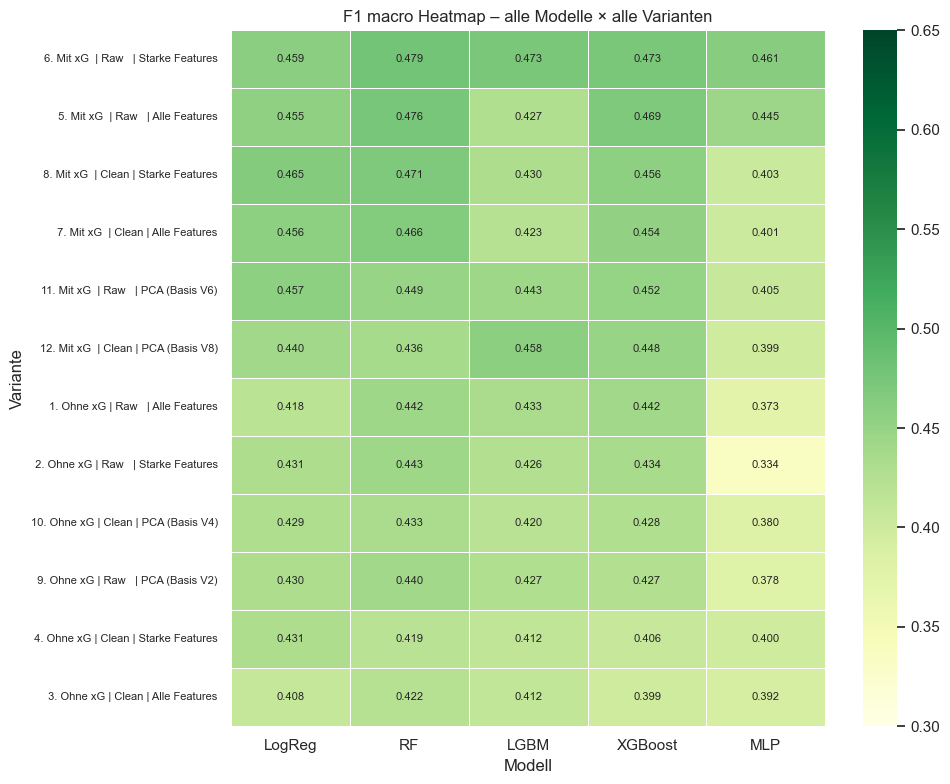
\includegraphics[width=\textwidth]{plots/plot_f1_heatmap.png}
    \caption{F1-macro-Heatmap aller fünf Modelle über alle zwölf
             Datensatzvarianten. Dunklere Grüntöne indizieren höhere
             F1-macro-Werte. xG-Varianten (obere sechs Zeilen) zeigen
             konsistent höhere Werte als Nicht-xG-Varianten.}
    \label{fig:f1-heatmap}
\end{figure}

\begin{figure}[h]
    \centering
    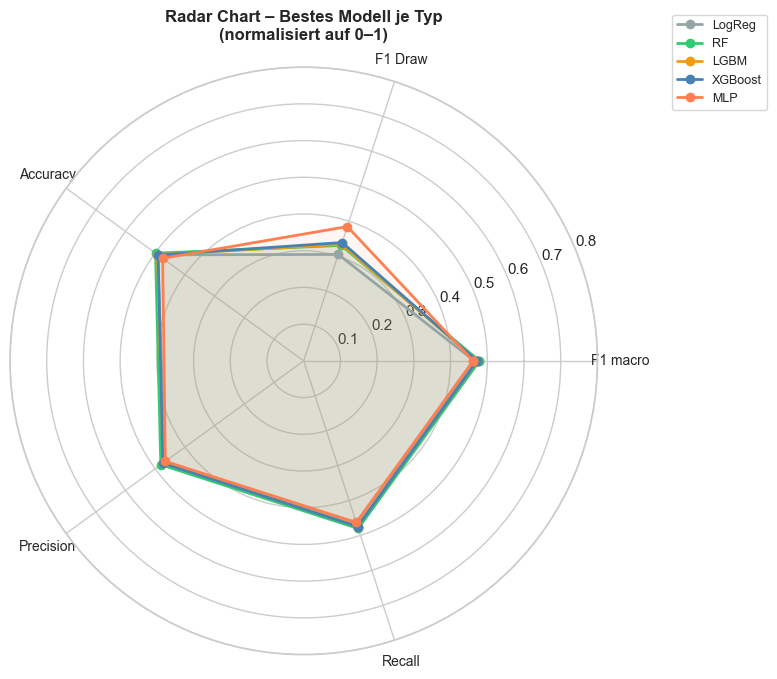
\includegraphics[width=0.65\textwidth]{plots/plot_radar.png}
    \caption{Radar-Chart der besten Modelle je Typ über fünf Metriken.
             Ein größeres Polygon entspricht einer besseren Gesamtleistung.}
    \label{fig:radar}
\end{figure}

\subsection{Zusammenfassung der Implementierung}

\begin{table}[h]
    \centering
    \caption{Zusammenfassung der Implementierungsparameter}
    \label{tab:impl-zusammenfassung}
    \begin{tabular}{l l l}
        \toprule
        \textbf{Komponente} & \textbf{Parameter} & \textbf{Wert / Begründung} \\
        \midrule
        EWA Span            & \texttt{span=10}     & $\alpha \approx 0{,}18$; neuere Spiele dominant \\
        IQR Multiplikator   & $c = 3{,}0$          & Nur extreme Ausreißer entfernen \\
        Korr.-Schwellenwert & $|\,r\,| > 0{,}1$    & Rauschen-freie Feature-Selektion \\
        PCA Varianz         & 95\,\%               & Multikollinearität reduzieren \\
        Train-Test-Split    & 80:20, stratifiziert & Repräsentative Klassenverteilung \\
        CV Folds            & 5                    & Stratified K-Fold \\
        Optimierungsmetrik  & F1 macro             & Robust bei Klassen-Imbalance \\
        Random Seed         & 42                   & Reproduzierbarkeit aller Läufe \\
        Gesamtläufe         & 60                   & 12 Varianten $\times$ 5 Modelle \\
        \bottomrule
    \end{tabular}
\end{table}